\chapter{基于图神经网络的流场模拟加速方法}

本章介绍了基于图神经网络的气动流场模拟加速方法,
首先利用CFD网格生成软件在算例几何模型上生成非结构网格,
基于网格单元拓扑连接信息、边界条件和初始条件提取图神经网络训练的输入数据;
利用CFD求解器获取图神经网络训练的真值。
然后基于图卷积神经网络设计了气动流场模拟加速模型,在模型训练完成后,
使用CFD求解器对气动流场模拟加速模型的输出结果进行优化。
最后在测试集上比较了气动流场模拟加速方法与传统CFD数值模拟方法的气动流场模拟效率。

\section{引言}

\subsection{动机分析}

利用深度学习方法对气动流场进行预测的主要思想是将气动流场模拟问题转化为图像回归预测问题,
因此需要将流场数据转化为矩阵的形式。
在处理流场中非结构数据时,则需要通过采样的方式将数据转化为结构规则的笛卡尔网格形式,
这样就会导致预测的结果在平滑区域(远场)过采样,而在流场边界层(几何体附近区域)欠采样,
导致预测流场结果在几何体周围轮廓模糊,不能真实的反映物理量在边界层的分布。
在传统基于网格的CFD模拟方法中,
一般通过加密边界层的网格密度以更加细致地捕捉边界层的速度和压力等物理量的变化,
使用均一的粗粒度的网格进行模拟根本不能得到准确的结果甚至导致计算不收敛。
此外,流场预测结果由深度学习模型输出,在复杂流动条件下,无法保证深度学习模型能够对流体运动规律进行准确学习,输出符合流体运动规律的预测结果。

基于以上考虑,本文在利用图神经网络进行流场模拟方面进行了探索,对气动流场模拟的效率和预测结果的有效性进行了权衡,
提出了基于图神经网络的流场模拟加速方法。

\subsection{研究思路}
与基于传统卷积神经网络的流场预测方法相比,基于图神经网络的流场模拟加速方法主要有两点不同:
1)流场数据表示方法通用性更强。
无论是结构网格还是非结构网格,利用图能够灵活地对网格单元的拓扑结构进行表示,
边界条件和初始条件可以处理为节点特征向量。
由于图结构利用网格对流场域进行了全尺寸模拟,不需要利用采样方法将流场表示为笛卡尔网格,
所以最大程度保留了原始流场数据中的信息,一些控制流体流动的全局变量也可以在图神经网络训练时用于每一个图节点上。
2)从根本上保证流场模拟结果的有效性。
利用CFD求解器对深度学习模型的预测结果进行优化,将计算收敛的结果作为最终的流场预测结果。
虽然深度学习模型在此方法中只是作为加速模块部分代替了CFD求解器的工作,
导致气动流场模拟效率低于基于深度学习的流场预测方法,
但由于气动流场模拟结果最终由CFD求解器输出,因此输出结果满足求解器计算收敛条件和流体流动物理规律。

由于图神经网络进行训练时需要保证图的拓扑结构保持不变,
因此本章主要针对给定几何外形在不同流动条件下气动流场模拟效率进行了研究。



\subsection{OpenFOAM网格数据结构}\label{meshstructure}
本文基于OpenFOAM软件进行网格生成和流场模拟。
OpenFOAM是基于C++程序语言开发用于场运算和操作的类库,主要包括两大类:求解器(solvers)和工具(utilities)。
用户可以根据特定的连续介质流体力学问题在标准的求解器基础上进行开发。工具主要有前处理工具和后处理工具两类。
前处理工具包括几何处理、网格处理、边界条件设置等,后处理工具包括数据提取与绘图、可视化处理等。
OpenFOAM主要网格文件及其包含的信息如表\ref{tab:openfoammesh}所示。

\begin{table}[htp]
	\setlength{\belowcaptionskip}{0.0cm}
	\caption{OpenFOAM网格文件信息}
	\label{tab:openfoammesh}
	\centering
	\begin{tabular}{c|c}
		\toprule
		文件 & 存储信息\\
		\midrule
		points  & 所有节点的三维坐标\\
		\midrule
		faces & 构造面单元的节点编号\\
		\midrule
		owner & 与面单元相对应owner体单元编号\\
		\midrule
		neighbour & 与面单元相对应neighbour体单元编号\\
		\midrule
		boundary & 边界条件设置\\		
		\bottomrule
	\end{tabular}
\end{table}

\texttt{points}文件以矢量场的形式存储所有节点坐标,单位为米,
文件主要内容如图\ref{fig:points_file}所示,节点的编号即为其坐标数据在points列表中的位置,初始编号为0。

\begin{figure}[htp]
	\centering
	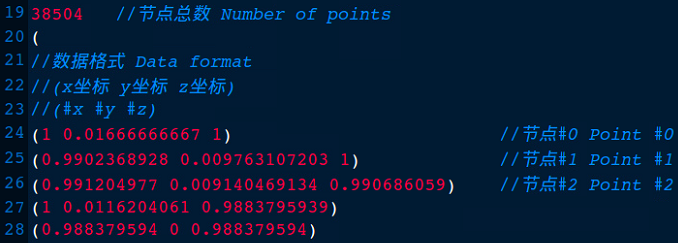
\includegraphics[width=0.72\textwidth]{./figures/points.png}
	\caption{points文件结构}
	\label{fig:points_file}	
\end{figure}

\texttt{faces}文件存储面单元-节点拓扑结构数据,文件主要内容如图\ref{fig:faces_file}所示。面单元最少由3个节点组成(三角形),其构造节点总数为每一行数据第一个整数(任意不小于3的值),每一行括号内的整数为面单元构造节点的编号,表示其在points列表中的位置。
面单元的编号即为数据在faces列表中的位置,初始编号为0。整个faces列表包含边界面单元。

\begin{figure}[htp]
	\centering
	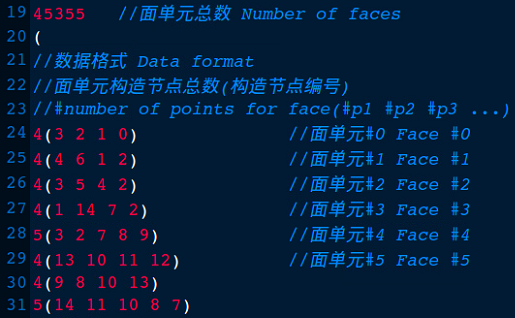
\includegraphics[width=0.72\textwidth]{./figures/faces.png}
	\caption{faces文件结构}
	\label{fig:faces_file}	
\end{figure}

如图\ref{fig:owner_neighbor}所示,owner体单元与neighbour体单元的标识基于公共面单元face外法向量($S_f$)的方向,即由owner单元指向neighbour单元。owner单元与neighbour单元有时亦被称为左单元与右单元。


\begin{figure}[htb]
	\centering
	\subfloat[]{\label{fig:on_2d}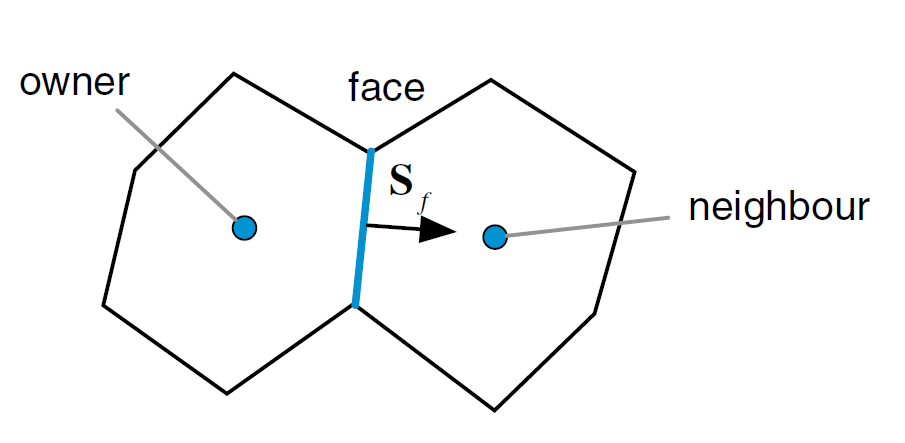
\includegraphics[width=0.45\textwidth]{figures/owner_neighbour_2d.png}} \qquad
	\subfloat[]{\label{fig:on_3d}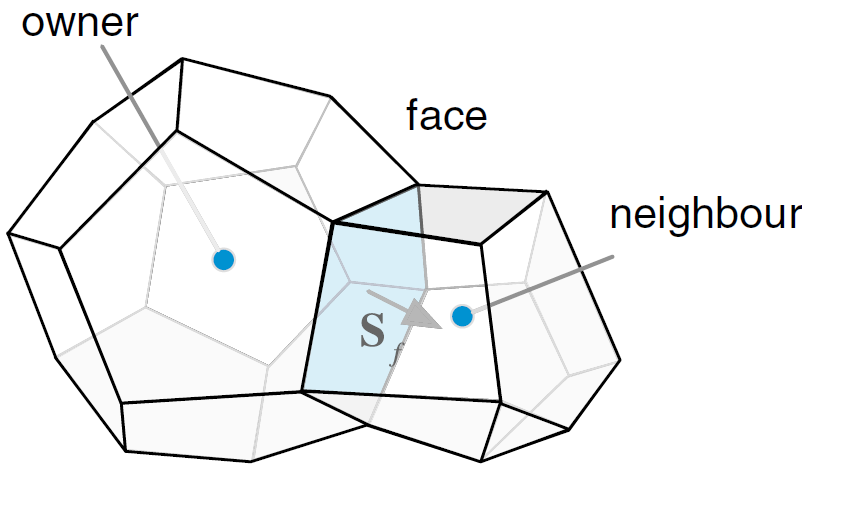
\includegraphics[width=0.45\textwidth]{figures/owner_neighbour.png}} 
	\caption{面的owner与neighbor的关系}
	\label{fig:owner_neighbor}
\end{figure}

\texttt{owner}文件存储owner单元-面单元拓扑结构数据,文件主要内容如图\ref{fig:owner_file}所示。owner列表存储相对应面单元的owner单元编号,初始编号为0,owner列表的位置对应面单元的编号,亦对应于其在faces列表中的位置。任何一个面单元总存在一个owner单元,因此owner单元总数与面单元总数nFaces相等。

\begin{figure}[htp]
	\centering
	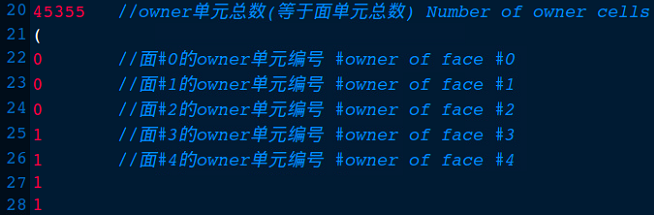
\includegraphics[width=0.72\textwidth]{./figures/owner.png}
	\caption{owner文件结构}
	\label{fig:owner_file}	
\end{figure}

\texttt{neighbour}文件存储neighbour单元-面单元拓扑结构数据,文件主要内容如图\ref{fig:neighbour_file}所示。neighbour列表存储相对应面单元的neighbour单元编号,初始编号不为0,neighbour列表的位置对应面单元的编号,亦对应于其在faces列表中的位置。需要特别说明的是,因为边界面单元没有neighbour单元,neighbour单元总数与内部面单元总数nInternalFaces相等。

\begin{figure}[htp]
	\centering
	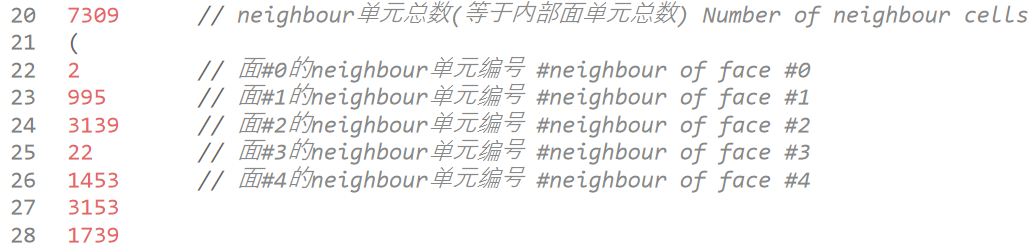
\includegraphics[width=0.72\textwidth]{./figures/neighbour.png}
	\caption{neighbour文件结构}
	\label{fig:neighbour_file}	
\end{figure}

\texttt{boundary}文件存储整个网格的边界信息,比如边界区域名称、边界类型type、面单元个数nFaces以及起始面单元编号startFace等,文件主要内容如图\ref{fig:boundary_file}所示。

\begin{figure}[htp]
	\centering
	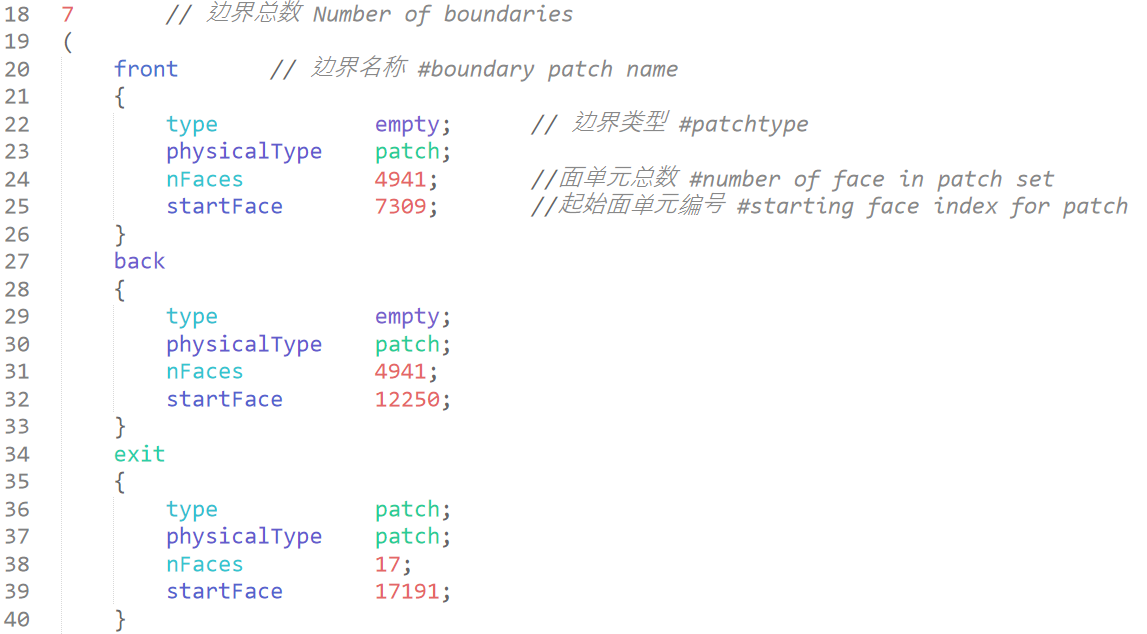
\includegraphics[width=0.72\textwidth]{./figures/boundary.png}
	\caption{boundary文件结构}
	\label{fig:boundary_file}	
\end{figure}

\noindent OpenFOAM不支持二维网格,对于导入的外部二维网格,OpenFOAM会自动给网格加一个厚度,然后将前后面(front和back)边界类型设置为空(empty)。


\section{基于GCN网络的气动流场模拟加速}

针对流场数据的非结构性和深度学习模型预测结果的可靠性,
本章提出了基于图卷积神经网络的气动流场模拟加速方法。
图\ref{fig:gcnflow}展示了基于GCN网络的气动流场加速方法的工作流程,主要包括三个部分:
a)图数据表示部分;b)基于GCN网络的气动流场加速部分;c)基于CFD求解器的模拟结果优化部分。

\begin{figure}[htp]
	\centering
	%\includegraphics[width=0.42\textwidth]{data/MLP.pdf}
	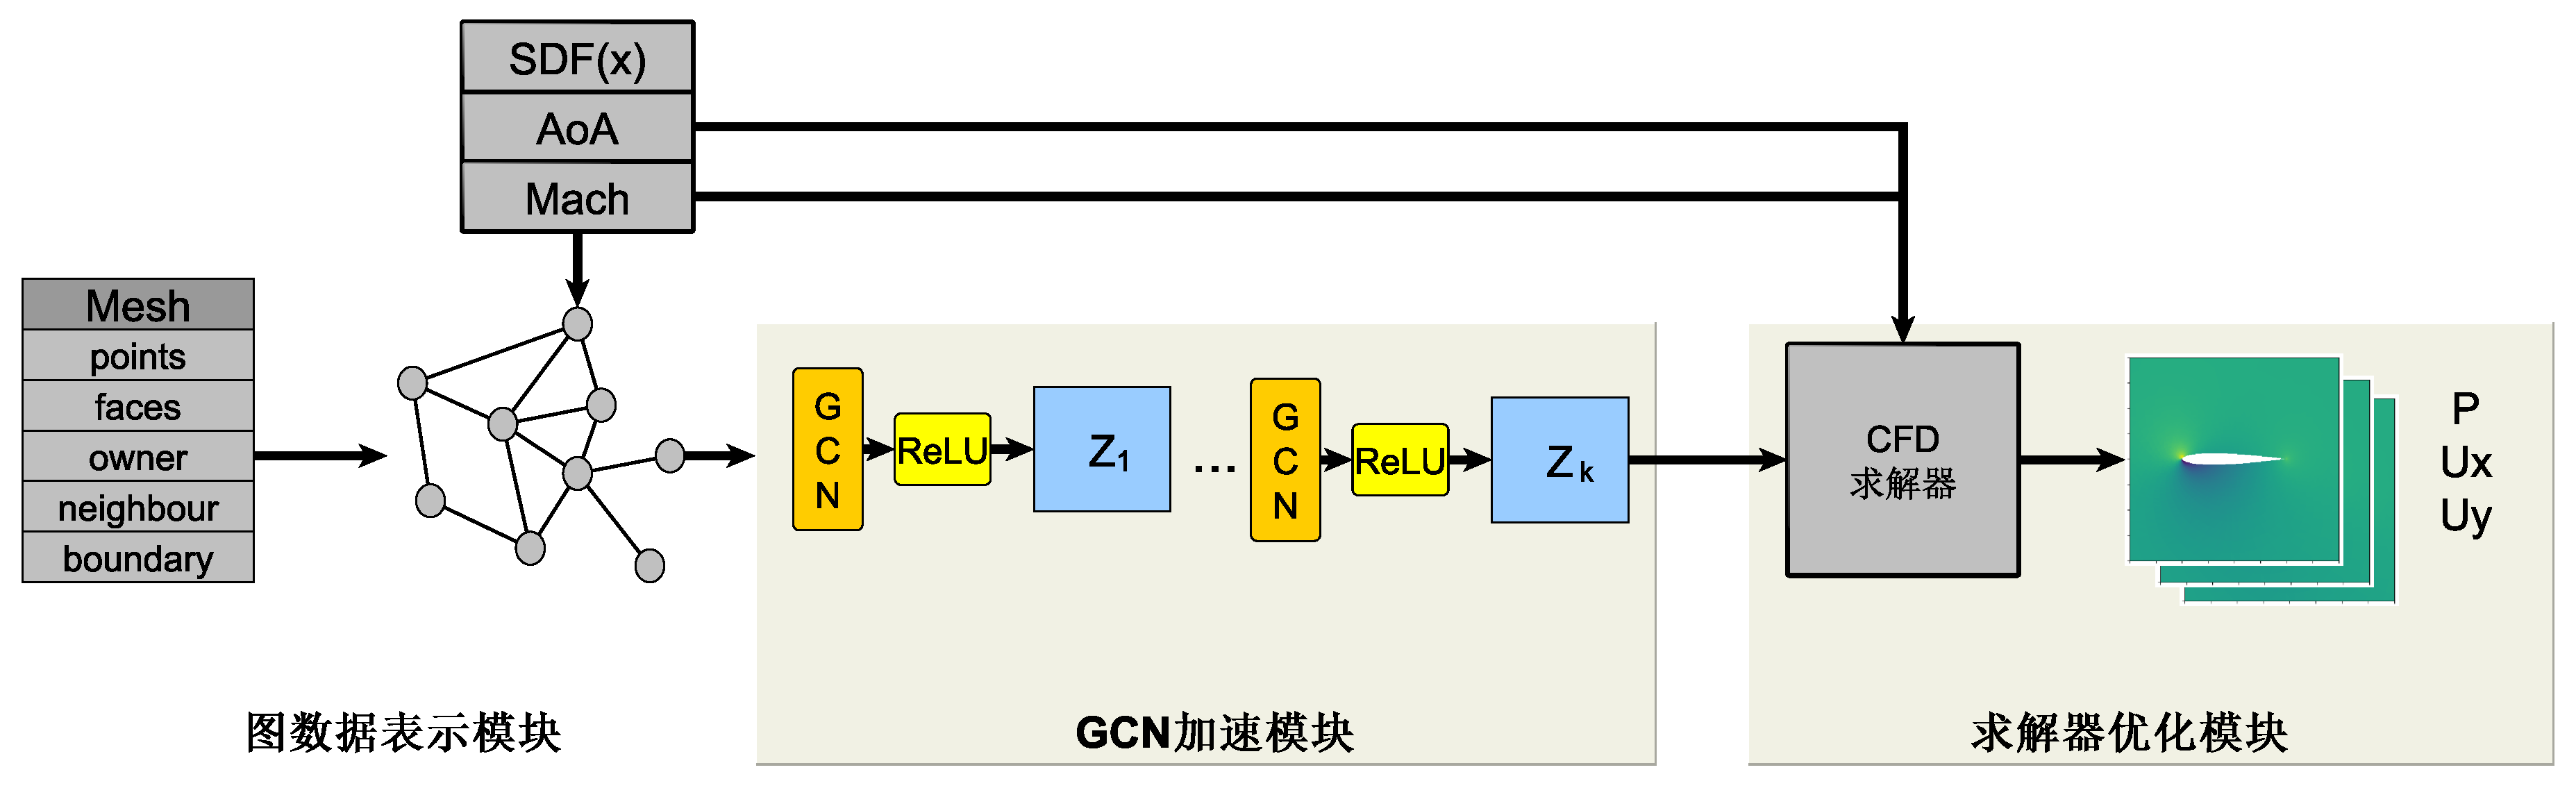
\includegraphics[width=0.99\textwidth]{figures/data/architecture2.pdf}
	\caption{基于GCN网络的气动流场加速方法示意图}
	\label{fig:gcnflow}
\end{figure}


\subsection{图结构数据表示}

本章定义图结构$G=\left(X, E\right)$来表示OpenFOAM网格信息,
其中$X \in R^{N \times d}$表示图节点,节点数目为N,节点特征维度为d。
$E$表示边,每条边连接两个图节点,考虑到流体在网格中是相互流通的,所有的边均定义为无向边。

不同于基于网格节点进行流场模拟的求解器SU2\cite{2015SU2},OpenFOAM是基于有限体积方法离散的求解器,
基于控制体单元进行流场计算和模拟。因此,每个节点对应网格中的体单元,节点数和体单元总数相同;
对于二维流场,节点特征值包括体心坐标($C_x$,$C_y$),体单元的边界属性()$B_l$。
其中体心坐标可以通过\texttt{points}文件中点坐标进行插值得到;
体单元的边界属性由\texttt{boundary}文件中所属面单元的边界类型决定。
此外,本章将更多流场信息嵌入图节点特征向量中,包括控制流体流动的马赫数(Mach)、攻角(AoA)等全局变量。
利用距离符号函数计算的给定图节点到几何边界的最短距离($D_s$),更好地帮助图神经网络学习节点的位置距离关系。
每条边对应两个体单元的共有面,边总数和内部面单元总数相同,两个体单元分别为该面单元的owner和neighbor。

通过以上表示可以得到基于体单元的图数据结构,
图节点$X=\left\{x_1, x_2 \ldots, x_n \right\}$,
每个图节点$X_i$的特征维度为6包括$C_x$,$C_y$,$B_l$,Mach,AoA和$D_s$;
边$E = \left\{e_1, e_2 \ldots, e_m \right\}$,
每条边$e_i$连接两个图节点$x_j,x_k \in X$且$j\not= k$。
这种基于网格结构的数据表示可以灵活处理各种复杂条件下的流场环境,
而且能够扩展到三维的流场数据表示,具有很强的通用性。
全局的流场控制信息可以通过特征向量嵌入的方式作用在每个图节点上,
与流场几何位置信息有效融合,充分参与图神经网络的训练。

\subsection{基于GCN网络的气动流场模拟加速}

利用图数据结构本章将流场数据表示为图神经网络可以接受的输入,
该图数据包括了网格结构信息、流场边界信息和流场控制条件信息等。
本章利用图卷积网络对形式化表示后的流场数据进行学习,输出流场稳定时速度场、压力场等相关物理量的预测结果。
算法\ref{GCNflow}展示了基于图卷积网络的气动流场模拟加速建模整体过程。

\renewcommand{\algorithmicrequire}{\textbf{输入:}}
\renewcommand{\algorithmicensure}{\textbf{输出:}}
\begin{algorithm}[htbp]
	\caption{基于图卷积网络的气动流场模拟加速建模}
	\label{GCNflow}
	\begin{algorithmic}[1]
		\REQUIRE 图数据结构:$Z_{0} = X = [C_x, C_y, B_l, AoA, Mach, D_s]$ 
		\ENSURE  二维气动流场模拟结果:$Y = [ U_x,U_y, P]$
		
		\STATE 构建图卷积网络模型,随机初始化权重矩阵
		\STATE 计算图形的拉普拉斯矩阵 L = D − W
		\STATE 定义图卷积操作GCN,确定激活函数
		\FOR{$i=1$ to $K-1$}
		\STATE $Z_{i} = \operatorname{ReLU}\left(\mathrm{GCN}_{i}\left(Z_{i-1}\right)\right) $
		\ENDFOR
		\STATE $Y_{temp} = \mathrm{GCN}_{K}\left(Z_{K-1}\right)$,$Y_{temp}$ = $[ U_x,U_y, P, nut, nuTilda]$
		\STATE $Y_{temp} \Rightarrow S_0$ 
		\STATE $Y = S_t = simpleFoam(S_0)$  
	\end{algorithmic}
\end{algorithm}

基于文献\cite{2016Semi}中的GCN模块,本章构建了用于气动流场模拟加速的图卷积网络,
包括$K$个图卷积层,前$K-1$个图卷积层后接一个激活层。
层与层之间的传播方式如下:
\begin{equation}
H^{(l+1)}=\sigma\left(\tilde{D}^{-\frac{1}{2}} \tilde{A} \tilde{D}^{-\frac{1}{2}} H^{(l)} W^{(l)}\right)
\end{equation}

\noindent 其中$H^{(l)} \in R^{N \times d^{(l)}}$是第$l$层图结构特征表达,维度是$N \times d^{(l)}$,
$N$表示图节点数目,$d^{(l)}$是节点特征维度。
矩阵$\tilde{A} = A + I$,其中A是图节点的邻接矩阵,I是单位矩阵,
表示每个节点在下一层状态不仅与自己的邻居有关还与节点本身有关。
矩阵$\tilde{D}$是$\tilde{A}$的度矩阵,用于归一化处理;
$W^{(l)}$是权重矩阵,在图卷积网络训练过程中不断调整;$\sigma$代表非线性激活函数ReLU。
图的拓扑结构在训练中保持不变,因此图卷积算子中$\tilde{D}^{-\frac{1}{2}} \tilde{A} \tilde{D}^{-\frac{1}{2}}$可以在训练之前确定并重复用于图卷积计算。

图卷积网络模型输出为$Y_{temp}$,包括$[ U_x,U_y, P, nut, nuTilda]$,
其中粘度系数nut和湍流运动粘度nuTilda是OpenFOAM模拟计算的中间结果,有助于构造CFD求解器的初始场。
结合流场控制条件攻角和马赫数,可以将气动流场预测结果转化为OpenFOAM中CFD求解器的初始场。
通过训练,GCN网络能够有效提取流场数据特征,学习流体流动规律;
在新的给定流场条件下,GCN网络能够输出一个接近真实模拟结果的预测流场。
因此,相对于传统CFD模拟,基于GCN的流场模拟方法在该预测结果的基础上在利用CFD求解器进行预测结果优化,
能够减少迭代计算的时间,从而实现模拟效率的提升。


\section{实验设置与结果分析}

\subsection{数据集与参数设置}

\subsubsection{基于OpenFOAM求解器生成数据集}
实验算例设置二维不可压湍流条件下固体外部流场,几何外形选取为空气动力学中经常研究的翼型。
机翼一般都有对称面。平行于机翼的对称面截得的机翼截面,称为翼剖面,通常也称为翼型。
翼型的几何形状是机翼的基本几何特性之一。
翼型的气动特性,直接影响到机翼及整个飞行器的气动特性,在空气动力学理论和飞行器设计中具有重要的地位。
图\ref{fig:airfoil_example}展示了翼型e342和翼型NACA 0012的几何外形示意图\cite{UIUCsite}。
\begin{figure}[htb]
	\centering
	\subfloat[e342]{\label{fig:e432}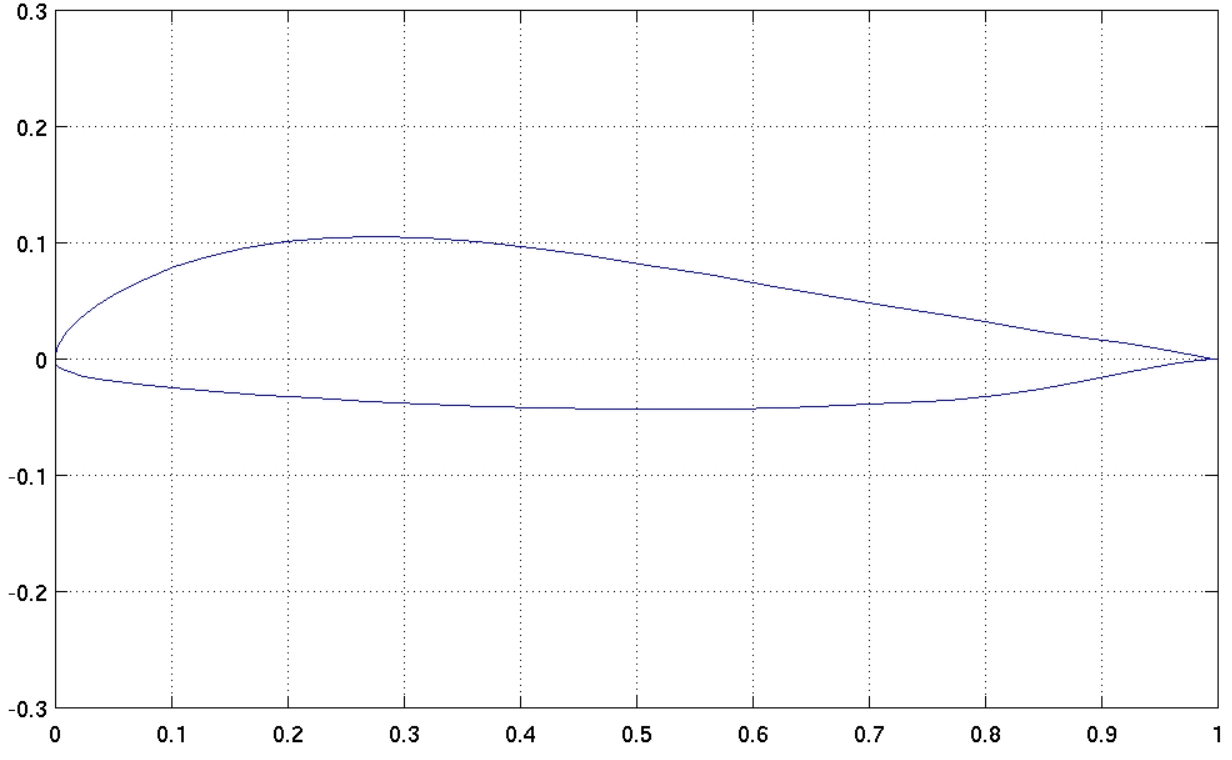
\includegraphics[width=0.42\textwidth]{figures/e342.png}} \qquad
	\subfloat[NACA 0012]{\label{fig:n0012}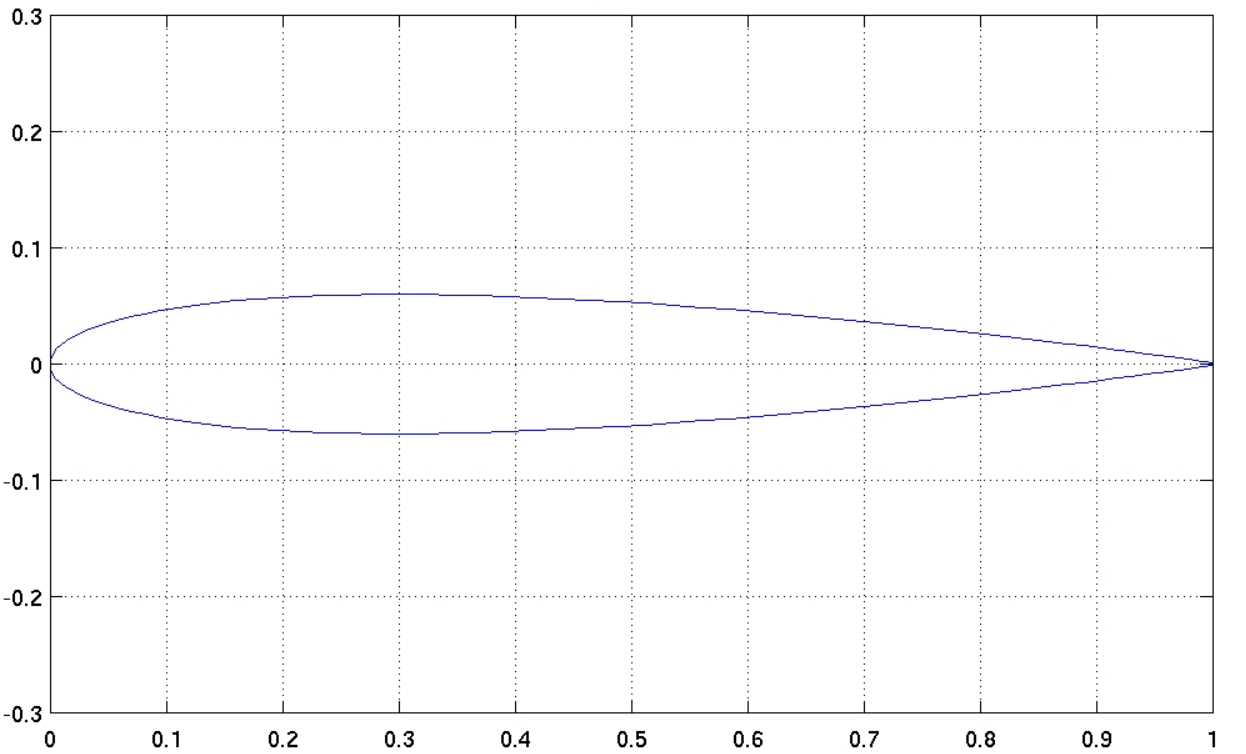
\includegraphics[width=0.42\textwidth]{figures/n0012.png}} 
	\caption{翼型e342和翼型NACA 0012几何外形示意图}
	\label{fig:airfoil_example}
\end{figure}

在获取翼型的几何模型之后,利用Gmsh\cite{gmsh}进行非结构网络的生成。
Gmsh是一个开源的具有内置CAD(Computer Aided Design)引擎和后期处理工具的三维有限元网格生成器,
可以方便地在Python脚本中调用Gmsh提供的接口对翼型进行网格生成。
全部网格信息保存在\texttt{.msh}文件中,再利用\texttt{gmshToFoam}指令将\texttt{.msh}文件导入OpenFOAM中,
就能得到\ref{meshstructure}节介绍的网格文件,完成网格生成任务。

\begin{figure}[htp]
	\centering
	%\includegraphics[width=0.42\textwidth]{data/MLP.pdf}
	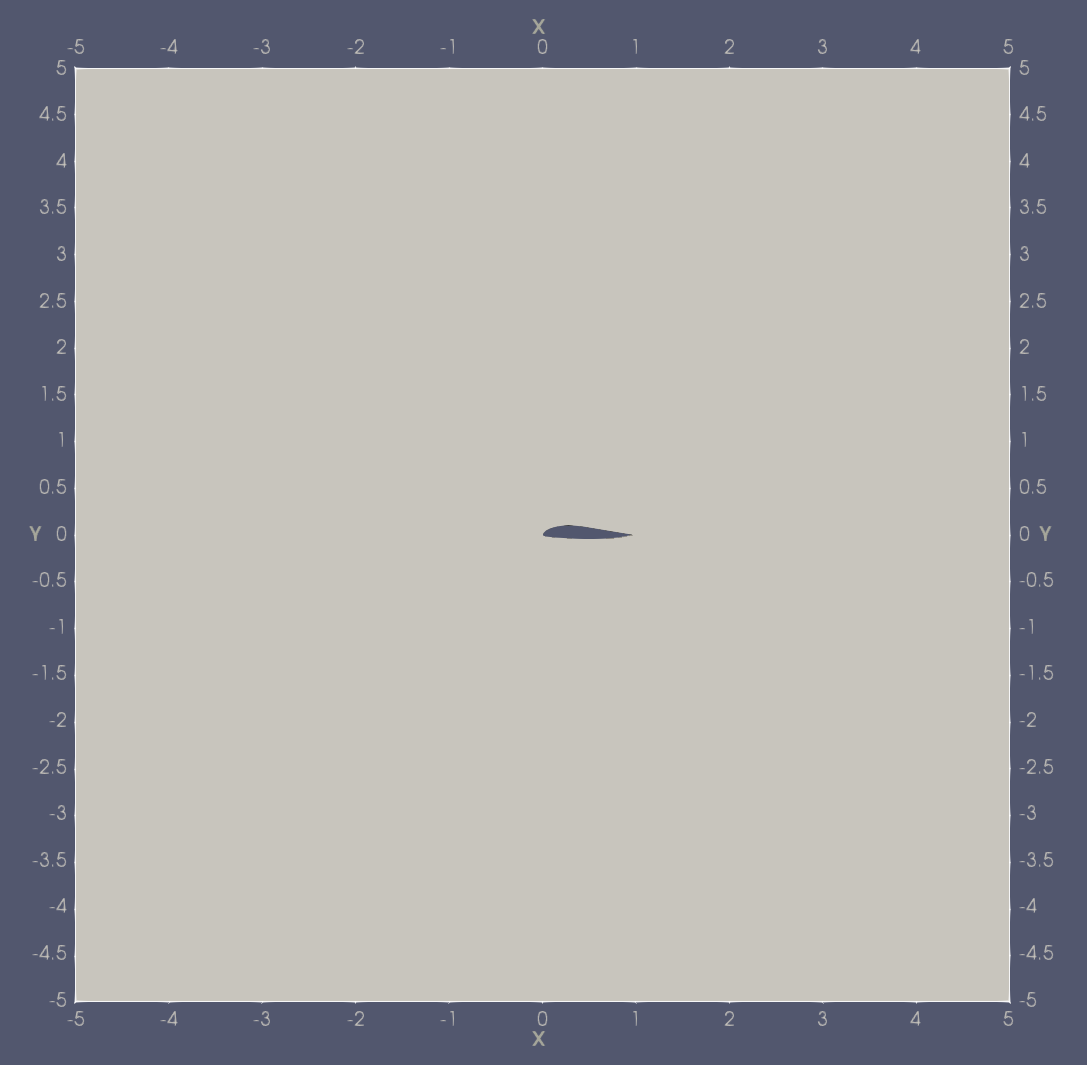
\includegraphics[width=0.42\textwidth]{figures/flowfield.png}
	\caption{实验算例二维流场区域示意图}
	\label{fig:field}
\end{figure}

在几何外形确定为翼型e342的基础上,本文在不同的攻角和来流马赫数条件下,利用OpenFOAM软件对翼型周围流场进行模拟。
图\ref{fig:field}展示了实验算例的流场区域设置,二维流场在x方向和y方向的范围均为-5\textasciitilde5,
翼型几何体长度范围0\textasciitilde1。
求解器使用OpenFOAM中不可压缩稳态流动求解器\texttt{simpleFoam},压力速度耦合采用的simple算法,湍流模型使用SA一方程模型。
计算的时间步长设置为1,迭代次数设置为5000保证在不同的流场条件下得到收敛的流场。
根据攻角(AoA)和流场来流马赫数(Mach  number)划分训练集和测试集,内插数据集和外推数据集划分如下:


\begin{equation}
\begin{array}{l}
\text {内插数据集:} \\
$$\text {AoA}_{train} =\{-10,-9, \ldots, 9,10\}$$ \\
$$\text {Mach}_{train} =\{0.2, 0.3, 0.35, 0.4, 0.5, 0.55, 0.6, 0.7\}$$ \\
$$\text {AoA}_{test} =\{-10,-9, \ldots, 9,10\}$$ \\ 
$$\text {Mach}_{test} =\{0.25, 0.45, 0.65\}$$
\end{array}
 \nonumber
\end{equation}

\begin{equation}
\begin{array}{l}
\text {外推数据集:} \\
$$\text {AoA}_{train} =\{-10,-9, \ldots, 9,10\}$$ \\
$$\text {Mach}_{train} =\{0.2, 0.25, 0.3, 0.35, 0.4, 0.45, 0.5, 0.55 \}$$ \\
$$\text {AoA}_{test} =\{-10,-9, \ldots, 9,10\}$$ \\ 
$$\text {Mach}_{test} =\{ 0.65, 0.6, 0.7\}$$
\end{array}
\nonumber
\end{equation}

通过${AoA}_{train}$和${Mach}_{train}$与${AoA}_{test}$和${Mach}_{test}$的组合分别构成训练集和测试集的流场条件,其中训练集样本大小为168,测试集数据大小为63。
在内插数据集中,训练集和测试集的数据不同,但是两个集合的参数有着相似的范围,
广泛用于流场模拟相关工作中\cite{bhatnagar2019prediction,DBLP:conf/kdd/GuoLI16}。
为了进一步测试基于GCN网络的流场模拟加速方法的泛化能力,本章设置了外推数据集,其测试集与训练集的马赫数分别处于不同的范围。



\subsubsection{参数设置}
本章在PyTorch深度学习框架下,基于PyTorch Geometric库提供的GCN模块设计了气动流场加速网络模型。
实验在Ubuntu18.04系统下利用GEFORCE RTX 2080Ti显卡进行。
模型训练使用Adam优化算法,学习率设置为$5\times10^{-5}$,模型在数据集上训练5000轮次(epoch)。
GCN网络训练损失函数使用常用的最小绝对值误差$L_1$损失函数。

在生成数据集和带回CFD求解器进行预测结果优化均使用OpenFOAM v7,
对于速度、压力和湍流运动粘度的残差收敛条件均设置为$1\times10^{-5}$。
在进行代数方程求解时,本章使用\texttt{GAMG}(generalised geometric-algebraic multi-grid)多重网格求解器对压力进行求解,
该求解器广泛用于加速CFD收敛;
速度和湍流运动粘度使用\texttt{smoothSolver}光滑求解器进行求解。所有求解器容错误差均为$1\times10^{-8}$,光滑器使用\texttt{GaussSeidel}。


\subsection{实验结果与分析}

本节将基于GCN模型的模拟结果称为$GCN$模拟结果;
将基于GCN模型的模拟结果并进一步利用CFD求解器进行优化的结果称为$GCN+CFD$模拟结果;
将传统的CFD求解器计算结果称为$P\_CFD$模拟结果。





\FIXME{更新数据}
\begin{figure}[htp]
	\centering
	%\includegraphics[width=0.42\textwidth]{data/MLP.pdf}
	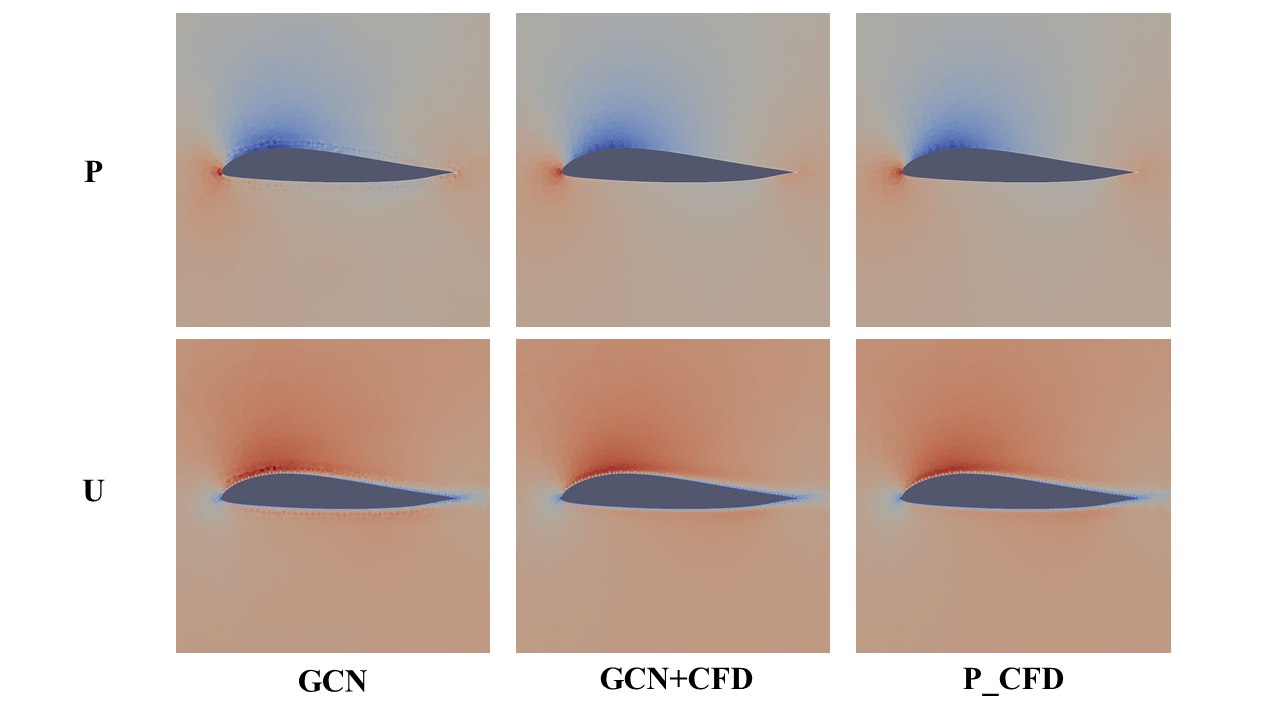
\includegraphics[width=0.88\textwidth]{figures/gcn_result/chapter4/gcncomp.png}
	\caption{内插数据集上速度场和压力场的模拟结果比较}
	\label{fig:interresult}
\end{figure}

\begin{figure}[htp]
	\centering
	%\includegraphics[width=0.42\textwidth]{data/MLP.pdf}
	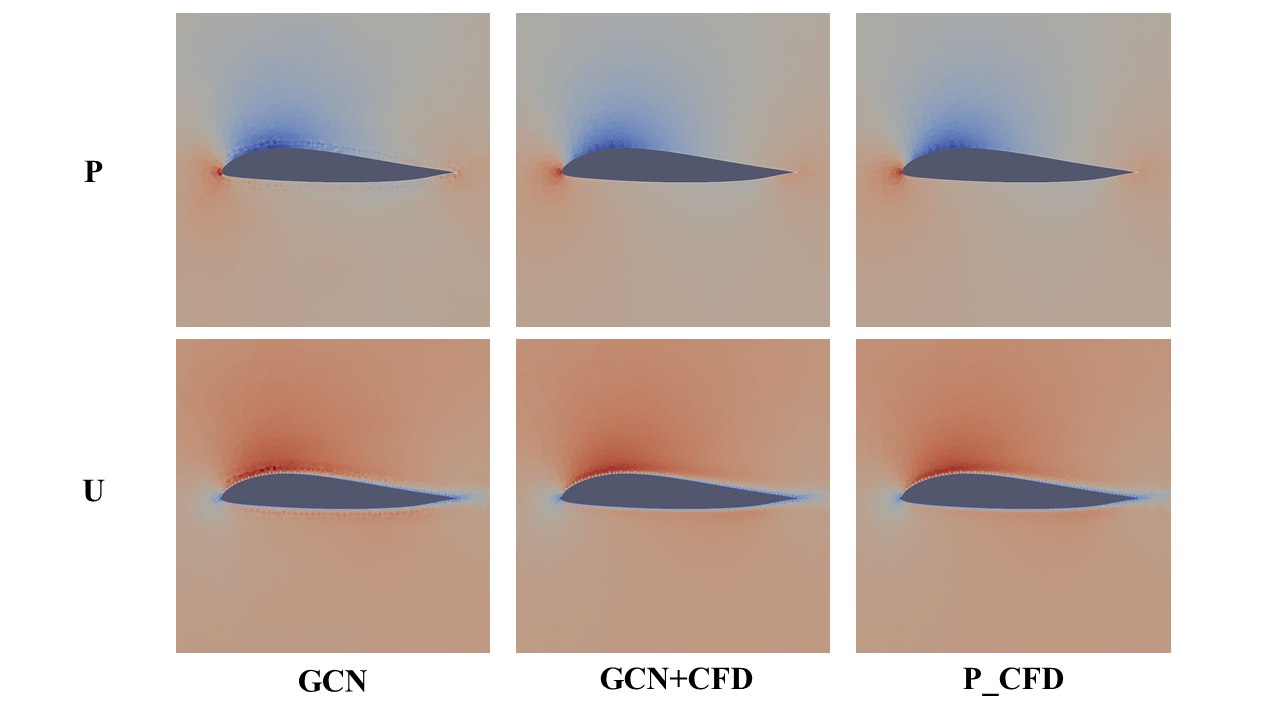
\includegraphics[width=0.88\textwidth]{figures/gcn_result/chapter4/gcncomp.png}
	\caption{外推数据集上速度场和压力场的模拟结果比较}
	\label{fig:outerresult}
\end{figure}


\begin{figure}[htp]
	\centering
	%\includegraphics[width=0.42\textwidth]{data/MLP.pdf}
	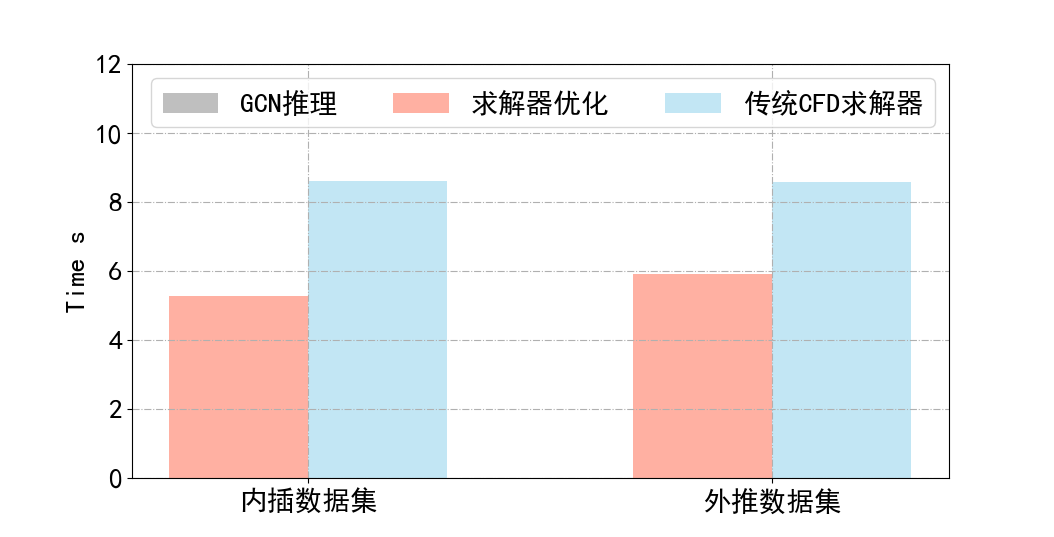
\includegraphics[width=0.88\textwidth]{figures/gcn_result/time.png}
	\caption{GCN+CFD方法在不同测试集上的模拟效率}
	\label{fig:timeresult}
\end{figure}





\section{本章小结}

